\documentclass{article}
\usepackage{iclr2026_conference,times}
\usepackage{hyperref}
\usepackage{url}
\usepackage{booktabs}
\usepackage{multirow}
\usepackage{graphicx}
\usepackage{xcolor}
\usepackage{tikz}
\usetikzlibrary{arrows.meta,positioning,fit,backgrounds}

\title{Who Prefers Structured Reasoning? \\
AI Judges Do, Domain Experts Don't}

% Anonymous submission
\author{Anonymous}

\newcommand{\fix}{\marginpar{FIX}}
\newcommand{\new}{\marginpar{NEW}}

%\iclrfinalcopy

\begin{document}

\maketitle

\begin{abstract}
Do LLM-as-judge improvements on synthesis tasks correspond to gains that domain experts actually perceive? We investigate by scaffolding LLM corpus analysis with operations drawn from human cognitive science---assumption excavation, absence detection, pattern induction, dialectical challenge---each formalized as a structured prompt. In experiments across three domains (machine learning, hand surgery, defense policy; $n{=}758$ documents), the scaffolded pipeline consistently outperforms a single-shot baseline under AI judges (+15.6\% to +32.0\%), confirmed by cross-model replication with GPT-5-family judges (+9.4\% to +25.3\%). However, three blinded domain experts did not reliably distinguish pipeline from baseline; the pipeline's strongest AI-judge dimension---assumption surfacing---was consistently perceived as stating field-obvious truths; and the experts interviewed requested navigation tools rather than better synthesis. This exposes a structural failure mode in rubric-based LLM-as-judge evaluation of synthesis: AI judges reward \textit{structural explicitness}---making implicit corpus features visible---while practitioners value \textit{epistemic novelty}---information they did not already know. The underlying principle is portable: what is implicit in a specialized corpus is largely what experts already know, so any system that mines implicit structure will rediscover the field's priors, and any rubric that rewards surfacing implicit structure will score this rediscovery as insight.
\end{abstract}

\section{Introduction}
\label{sec:intro}

LLM-as-judge evaluation is increasingly used to validate synthesis systems \citep{zheng2023judging,shankar2024validates,bavaresco2024llms}. But synthesis is reader-relative: quality depends on what the reader already knows. This paper asks whether rubric-based AI judge improvements on corpus synthesis tasks correspond to gains that domain experts actually perceive---and demonstrates that they do not.

Human experts routinely decompose analytical reasoning into distinct cognitive operations: identifying patterns, surfacing assumptions, detecting absences, constructing counterarguments \citep{polya1945solve,sternberg1985componential,newell1972human}. We scaffold LLM corpus analysis with this approach, formalizing five such operations as structured prompts that each target a distinct epistemic dimension (\S\ref{sec:framework}). The design extends structured prompting \citep{wei2022chain,zhou2023leasttomost,khot2023decomposed} from single-problem reasoning to multi-operation epistemic workflows over document collections, drawing on cognitive architectures \citep{anderson2004integrated} that model cognition as compositions of modular operations. Synthesis is one downstream application of these operations; others---planning, hypothesis generation, evaluation---remain untested.

Applied to synthesis, the pipeline produces large, consistent AI judge gains across three unrelated domains (+15.6\% to +32.0\%), confirmed by cross-model replication with GPT-5-family judges (+9.4\% to +25.3\%). It is, by standard LLM-as-judge methodology, a clear improvement. Yet three blinded domain experts did not reliably distinguish pipeline from baseline, and the pipeline's strongest AI-judge dimension---assumption surfacing---was consistently perceived as stating field-obvious truths. This exposes a structural failure mode: AI judges reward \textit{structural explicitness}---making implicit corpus features visible---while practitioners value \textit{epistemic novelty}---information they did not already know. The underlying principle is that what is implicit in a specialized corpus is largely what experts already know; mining implicit structure therefore rediscovers the field's priors, and rubrics that reward surfacing implicit structure score this rediscovery as insight.

Our contributions are: (1)~evidence of a structural failure mode in LLM-as-judge evaluation of synthesis tasks, where judge-preferred outputs are indistinguishable to domain experts; (2)~a portable principle---what is implicit in a specialized corpus is largely what experts already know---with implications for any evaluation regime that rewards structural explicitness; (3)~a cognitively-motivated decomposition of corpus analysis into modular epistemic operations, whose outputs produce reliable, cross-model AI judge gains and whose intermediate artifacts may have standalone utility beyond synthesis (\S\ref{sec:discussion}).

\section{Related Work}
\label{sec:related}

\textbf{LLM-as-judge reliability} \citep{zheng2023judging,shankar2024validates,bavaresco2024llms} is an active concern, with growing evidence that judge preferences diverge from human preferences on open-ended tasks; we contribute evidence for a specific failure mode on synthesis tasks where AI judges and domain experts evaluate along fundamentally different axes. \textbf{Structured prompting} decomposes complex tasks into intermediate steps \citep{wei2022chain,zhou2023leasttomost,khot2023decomposed,yao2023tree}; we extend this to multi-operation epistemic workflows over document collections, using the resulting pipeline as a controlled probe for studying evaluation divergence. \textbf{Multi-agent LLM systems} \citep{du2024improving,liang2023encouraging,wu2023autogen,hong2024metagpt,zhang2024chain} improve outputs through cognitive diversity; our pipeline implements diversity through orthogonal \textit{operations} rather than competing agents. \textbf{Cognitive architectures} \citep{anderson2004integrated,laird2012soar,sumers2024cognitive,binz2023turning} model cognition as compositions of modular operations; we operationalize this for LLM corpus analysis. \textbf{LLM-based synthesis} \citep{wang2024autosurvey,lu2024aiscientist,giglou2025llms4synthesis,si2024can} typically uses LLMs as summarizers; we use cognitively-inspired analytical operations that generate epistemic artifacts (assumption trees, gap maps, antitheses) as context for synthesis.

\section{Framework and Experimental Design}
\label{sec:framework}

\subsection{Epistemic Operations}

We identify five core operations, each targeting a distinct reasoning faculty (detailed descriptions in Appendix~\ref{app:operations}). Three operate on the full corpus; two operate on a stratified random subset of 30 documents:

\begin{enumerate}
    \item \textbf{Inductify} (pattern induction): Extract non-obvious structural commonalities across documents. \textit{[full corpus]}
    \item \textbf{Negspace} (absence detection): Identify what is conspicuously missing from the corpus. \textit{[full corpus]}
    \item \textbf{Handlize} (operational extraction): Retain only claims with operational grip. \textit{[full corpus]}
    \item \textbf{Excavate} (assumption archaeology): Uncover implicit premises in individual documents. \textit{[30-doc subset]}
    \item \textbf{Antithesize} (dialectical challenge): Generate the strongest opposition to excavated assumptions. \textit{[from excavate output]}
\end{enumerate}

These compose into a directed pipeline (Figure~\ref{fig:pipeline}). Critically, the final synthesis prompt is \textit{identical} between baseline (Condition~A) and pipeline (Condition~C)---the only variable is whether structured operation outputs are prepended as context.

\begin{figure}[t]
\centering
\begin{minipage}[t]{0.30\linewidth}
\centering
\textbf{Baseline (A)}\\[2pt]
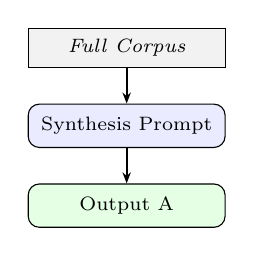
\begin{tikzpicture}[
    node distance=0.45cm,
    op/.style={draw, rounded corners, fill=blue!8, minimum width=2.5cm, minimum height=0.55cm, font=\scriptsize},
    data/.style={draw, fill=gray!10, minimum width=2.5cm, minimum height=0.5cm, font=\scriptsize\itshape},
    arr/.style={-{Stealth[length=1.4mm]}, thick},
]
\node[data] (corpusA) {Full Corpus};
\node[op, below=of corpusA] (promptA) {Synthesis Prompt};
\node[op, below=of promptA, fill=green!10] (outA) {Output A};
\draw[arr] (corpusA) -- (promptA);
\draw[arr] (promptA) -- (outA);
\end{tikzpicture}
\end{minipage}
\hfill
\begin{minipage}[t]{0.66\linewidth}
\centering
\textbf{Pipeline (C)}\\[2pt]
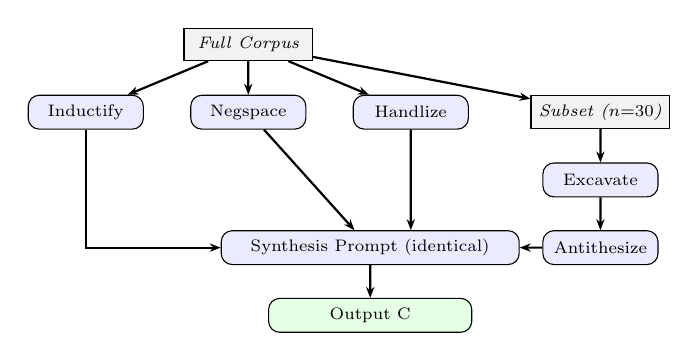
\begin{tikzpicture}[
    scale=0.86,
    transform shape,
    node distance=0.45cm and 0.55cm,
    op/.style={draw, rounded corners, fill=blue!8, minimum width=1.7cm, minimum height=0.5cm, font=\scriptsize},
    data/.style={draw, fill=gray!10, minimum width=1.9cm, minimum height=0.48cm, font=\scriptsize\itshape},
    arr/.style={-{Stealth[length=1.4mm]}, thick},
]
\node[data] (corpusC) at (0,0) {Full Corpus};
\node[op] (ind) at (-2.4,-1.0) {Inductify};
\node[op] (neg) at (0.0,-1.0) {Negspace};
\node[op] (hand) at (2.4,-1.0) {Handlize};
\node[data] (subset) at (5.2,-1.0) {Subset ($n{=}30$)};
\node[op] (exc) at (5.2,-2.0) {Excavate};
\node[op] (anti) at (5.2,-3.0) {Antithesize};
\node[op, minimum width=4.4cm] (promptC) at (1.8,-3.0) {Synthesis Prompt (identical)};
\node[op, fill=green!10, minimum width=3.0cm] (outC) at (1.8,-4.0) {Output C};
\draw[arr] (corpusC) -- (ind);
\draw[arr] (corpusC) -- (neg);
\draw[arr] (corpusC) -- (hand);
\draw[arr] (corpusC) -- (subset);
\draw[arr] (subset) -- (exc);
\draw[arr] (exc) -- (anti);
\draw[arr] (ind) |- (promptC);
\draw[arr] (neg) -- (promptC);
\draw[arr] (hand) -- (hand |- promptC.north);
\draw[arr] (anti) -- (promptC);
\draw[arr] (promptC) -- (outC);
\end{tikzpicture}
\end{minipage}
\caption{Both conditions use the same synthesis prompt. The pipeline prepends structured intermediate outputs as additional context before invoking that shared prompt.}
\label{fig:pipeline}
\end{figure}

\subsection{Experimental Setup}

We compare Conditions A and C across three domains chosen for maximal diversity (Table~\ref{tab:corpora}). Both use Claude Opus 4.6 \citep{anthropic2025claude} for generation. AI judge evaluation uses 3 independent judge instances on 6 dimensions (1--5 scale; Appendix~\ref{app:rubric}). To control for same-model bias, we run a full independent replication with Codex (GPT-5-family) judges using the identical rubric. Human expert evaluation uses blinded paired outputs with randomized labels, one domain expert per domain. Statistical comparisons use Wilcoxon signed-rank tests on run-level paired means, with 95\% bootstrap confidence intervals (10,000 resamples, seed=42) and Cohen's $d$ (pooled SD). Full details are in Appendix~\ref{app:experimental}.

\begin{table}[t]
\caption{Experimental corpora.}
\label{tab:corpora}
\begin{center}
\begin{tabular}{lllrl}
\toprule
\textbf{Conference} & \textbf{Domain} & \textbf{Year} & \textbf{$n$} & \textbf{Type} \\
\midrule
ICLR & Machine learning & 2025 & 213 & Oral abstracts \\
AAHS & Hand surgery & 2026 & 218 & Podiums + ePosters \\
AUSA & Defense policy & 2025 & 327 & News/policy articles \\
\bottomrule
\end{tabular}
\end{center}
\end{table}

\section{Results}
\label{sec:results}

\subsection{AI Judges: Opus and Codex Both Favor the Pipeline}

The pipeline consistently outperforms the baseline across all three domains under Claude Opus 4.6 judges (Table~\ref{tab:crossdomain_opus}), with large effect sizes ($d{=}1.98$--$2.44$; pooled $\Delta{=}+5.35$, $p{<}.001$, Wilcoxon signed-rank on run-level paired means; 95\% bootstrap CIs exclude zero in all cases). Scores near the ceiling should be interpreted cautiously.

\begin{table}[t]
\caption{Cross-domain Opus judge results (mean totals, /30 scale). CIs are 95\% bootstrap (10k resamples); $d$ is Cohen's $d$ (pooled); $p$ is Wilcoxon signed-rank on run-level paired means.}
\label{tab:crossdomain_opus}
\begin{center}
\begin{tabular}{lccccccc}
\toprule
\textbf{Domain} & \textbf{A} & \textbf{C} & \textbf{$\Delta$} & \textbf{95\% CI} & \textbf{$d$} & \textbf{$p$} & \textbf{$n$} \\
\midrule
ICLR 2025 & 20.87 & 27.53 & +6.67 & [3.5, 9.8] & 1.98 & .031 & 5 \\
AAHS 2026 & 23.47 & 27.13 & +3.67 & [2.1, 5.3] & 2.44 & .031 & 5 \\
AUSA 2025 & 21.22 & 27.56 & +6.33 & [6.0, 6.7] & --- & .125 & 3 \\
\midrule
\textit{Pooled} & 21.89 & 27.24 & +5.35 & [3.9, 7.1] & 2.19 & ${<}.001$ & 13 \\
\bottomrule
\end{tabular}
\end{center}
\end{table}

To address the concern that same-model judges may inflate the pipeline's advantage, we ran a full independent replication with Codex (GPT-5-family) judges using the same six-dimension rubric (Table~\ref{tab:crossdomain_codex}). The pipeline advantage holds under the cross-model judge on all three domains (pooled $\Delta{=}+3.87$, $p{<}.001$), at approximately 72\% of the Opus effect size. Assumption surfacing remains the largest per-dimension gain under both judge families (Table~\ref{tab:dimensions_codex} in Appendix).

\begin{table}[t]
\caption{Cross-domain Codex (GPT-5-family) replication (mean totals, /30 scale). Per-dimension breakdowns in Appendix~\ref{app:scores}.}
\label{tab:crossdomain_codex}
\begin{center}
\begin{tabular}{lccccccc}
\toprule
\textbf{Domain} & \textbf{A} & \textbf{C} & \textbf{$\Delta$} & \textbf{95\% CI} & \textbf{$d$} & \textbf{$p$} & \textbf{$n$} \\
\midrule
ICLR 2025 & 21.08 & 26.42 & +5.33 & [2.8, 7.8] & 2.25 & .063 & 4 \\
AAHS 2026 & 25.40 & 27.80 & +2.40 & [1.5, 3.3] & 2.59 & .031 & 5 \\
AUSA 2025 & 23.78 & 28.56 & +4.78 & [4.3, 5.3] & --- & .125 & 3 \\
\midrule
\textit{Pooled} & 23.69 & 27.56 & +3.87 & [2.8, 5.0] & 2.08 & ${<}.001$ & 12 \\
\bottomrule
\end{tabular}
\end{center}
\end{table}

The dimensional profile is consistent across both judge sets: \textbf{assumption surfacing} is the largest gain in all three domains under Opus (+1.33 to +2.00) and a top gain under Codex (+1.00 to +1.56). The pipeline also acts as a \textbf{variance reducer}: on ICLR, Condition~C has SD~=~0.7 across 5 runs while Condition~A shows bimodal variance (SD~=~4.5), with catastrophic quality drops on 2 of 5 runs (Figure~\ref{fig:variance} in Appendix).

Notably, the Codex judges detect a tradeoff invisible to Opus: on AAHS, the pipeline's corpus coverage ($-$0.73) and decision-readiness ($-$0.60) \textit{decrease} relative to baseline---the pipeline gains epistemic depth at the cost of breadth and actionability. This finding independently corroborates the human experts' critique (\S\ref{sec:human}).

(Appendix~\ref{app:scores} reports an ablation study suggesting a non-additive interaction between operations.)

\subsection{Human Experts: No Perceived Difference}
\label{sec:human}

The AI judge results present a clear pipeline advantage. Blinded domain experts tell a different story. Full reviewer transcripts are in Appendix~\ref{app:human_detail}.

\paragraph{Defense policy (AUSA 2025).} The reviewer perceived the pipeline's interpretive additions as obvious:

\begin{quote}
``Of course AUSA does advocacy. Of course nobody says China is the adversary. Of course they don't talk about DOGE and piss off the admin.''
\end{quote}

If the interpretation is bad, ``I only want the facts, and the naive one sticks to the facts.'' The gaps flagged by the pipeline ``aren't the ones that an expert would want flagged.''

\paragraph{Hand surgery (AAHS 2026).} The reviewer reported: ``honestly the 2 were similar.'' Neither output provided information beyond existing knowledge: ``Nothing new or informative for me\ldots\ It serves as a reinforcement of what I presumed to be.''

\paragraph{Machine learning (ICLR 2025).} The reviewer found ``one isn't obviously `better' than the other'' with differences ``mostly about taste.'' Trajectory predictions were ``mostly obvious conclusions.'' The overall assessment: ``I don't know if I'd have found them helpful beyond it being a cute summarization.''

Critically, this reviewer articulated what experts \textit{actually} wanted: outlier highlighting (``the `weird' and therefore possibly more interesting papers''), personalized relevance filtering, temporal comparison with prior years, and---most strikingly---the pipeline's \textit{intermediate} analytical outputs as standalone products: ``It'd almost be helpful to have excavate or ramify outputs on the corpus as a whole.''

\subsection{The Divergence}

Three evaluator populations form a gradient of decreasing enthusiasm (Table~\ref{tab:divergence}):

\begin{table}[t]
\caption{AI judge vs.\ human expert evaluation: a qualitative comparison.}
\label{tab:divergence}
\begin{center}
\small
\begin{tabular}{p{2.1cm}p{2.3cm}p{3.8cm}}
\toprule
\textbf{Opus judges} & \textbf{Codex judges} & \textbf{Human experts} \\
\midrule
Pipeline clearly superior (+16--32\%) & Pipeline moderately superior (+9--25\%) & ``The 2 were similar''; differences are ``taste'' \\
\addlinespace
Assumption surfacing: largest gain (+1.33 to +2.00) & Assumption surfacing: largest gain (+1.00 to +1.56) & Assumptions surfaced are ``of course'' truths \\
\addlinespace
No tradeoffs detected & Detects coverage and actionability tradeoff & Experts want navigation, not synthesis \\
\bottomrule
\end{tabular}
\end{center}
\end{table}

\textbf{(1)~No interviewed expert distinguished conditions.} No reviewer identified one output as clearly superior. \textbf{(2)~The pipeline's strongest AI-judge dimension is its weakest human dimension.} Assumption surfacing---the largest AI judge gain under both model families---was uniformly perceived as stating known truths. \textbf{(3)~The interviewed experts wanted navigation, not synthesis.} Reviewers wanted personalized filtering, temporal comparisons, anomaly highlighting, and raw analytical artifacts rather than polished reports. \textbf{(4)~Cross-model judges form a gradient.} The Codex judges' intermediate position---confirming the pipeline advantage but at smaller magnitude while detecting actionability tradeoffs---suggests that even within AI evaluation, the measured effect depends on what the judge attends to.

\section{Discussion}
\label{sec:discussion}

\paragraph{A structural failure mode in synthesis evaluation.} The central finding is not a calibration error but a divergence in what evaluation regimes optimize for. AI judges reward \textit{structural explicitness}---making implicit corpus features visible: unstated assumptions, missing topics, cross-document patterns. The experts interviewed valued \textit{epistemic novelty}---information that changes what they know or what they would do. The pipeline reliably maximizes the first while failing to move the second, and the cross-model replication confirms this is not a same-model artifact. Assumption surfacing---the pipeline's largest AI judge gain---illustrates the mechanism: what is implicit in a specialized corpus is largely what experts already know. ``Of course AUSA does advocacy'' is not an insight; it is the ground on which all analysis stands. Any evaluation regime that rewards surfacing implicit structure will score this rediscovery of priors as insight.

\paragraph{Intermediate artifacts as the product.} The ML reviewer's request for the pipeline's intermediate outputs as standalone products inverts the architecture: the analytical intermediates may have more standalone utility than their composition, suggesting reorientation from synthesis to analytical infrastructure.

\paragraph{Implications for LLM-as-judge evaluation.} On well-defined tasks, LLM judges correlate well with human preferences \citep{zheng2023judging}. But synthesis is inherently underspecified---``different people will have wildly different preferences.'' No rubric that ignores the reader's prior knowledge can measure whether a synthesis tells them something new. For synthesis evaluation, the reader's expertise is not a confound to control for; it is the variable that determines utility.

\paragraph{Beyond synthesis.} The cross-model replication confirms the pipeline produces detectably different, more epistemically structured text---but synthesis may not be the downstream task where that structure is most valuable. The cognitive operations that compose the pipeline (assumption excavation, absence detection, pattern induction) have natural applications in planning, hypothesis generation, and evaluation, where the structural artifacts might constitute the product rather than context for a separate generation step. Whether the AI-judge/expert divergence persists for these tasks is an open question.

\paragraph{Limitations.} Three experts (one per domain) is standard for expert evaluation but insufficient for population-level inference. Active practitioners may be biased toward finding corpus themes ``obvious''---less experienced readers (e.g., graduate students, adjacent-field researchers) might value assumption surfacing more, and a larger-$n$ study stratified by expertise level would test whether the divergence scales with domain familiarity. Our AI judge evaluation uses two model families (Claude Opus and GPT-5 Codex), both closed-weight frontier models; replication with open-weight models (e.g., Llama, Mixtral) and smaller-scale systems would clarify whether the structural-explicitness bias is a property of scale, RLHF training, or rubric-following capability more broadly. The same-model concern---Opus serves as both generator and judge---is partially mitigated by the Codex replication, but a design where no judge family overlaps with the generator would be stronger.

\section{Conclusion}

We demonstrate a structural failure mode in LLM-as-judge evaluation of synthesis tasks: a pipeline that produces large, cross-model AI judge gains ($p{<}.001$ pooled under both Opus and Codex) is invisible to domain experts. The mechanism is portable: what is implicit in a specialized corpus is largely what experts already know, so any evaluation regime that rewards structural explicitness will score the rediscovery of field priors as insight. Synthesis evaluation without a model of the reader's prior knowledge cannot distinguish explicitness from genuine insight.

\subsubsection*{Reproducibility}

All code, configurations, prompts, and raw scores are available upon request. Experiments are fully deterministic given a fixed random seed; hosted-model nondeterminism may introduce residual variation.

\subsubsection*{Acknowledgments}
Removed for anonymous review.

\bibliography{references}
\bibliographystyle{iclr2026_conference}

%% ============================================================
%% APPENDIX
%% ============================================================
\appendix

\section{Epistemic Operation Descriptions}
\label{app:operations}

\begin{enumerate}
    \item \textbf{Inductify} (pattern induction): Extract non-obvious structural commonalities across documents---shared constraints, latent mechanisms, and convergent findings that would not be visible from any single document. Operates on the full corpus.
    \item \textbf{Negspace} (absence detection): Across the corpus, identify what \textit{should} be present given the statistical structure of the collection but is conspicuously absent---missing conclusions, unexamined premises, absent populations or methods. Operates on the full corpus.
    \item \textbf{Handlize} (operational extraction): Strip rhetorical mass from each document, retaining only the claims, findings, and methods with operational grip---what a practitioner could act on, cite, or build from. Operates on the full corpus.
    \item \textbf{Excavate} (assumption archaeology): For individual documents in a stratified random subset of 30, uncover the implicit premises that must be true for the stated conclusions to hold. Identify cruxes---assumptions where, if wrong, the entire edifice shifts.
    \item \textbf{Antithesize} (dialectical challenge): Given the excavated assumptions, generate the strongest possible opposition---not as refutation, but as an alternative complete perspective that identifies where shared assumptions are weakest.
\end{enumerate}

These operations are orthogonal: inductify asks ``what recurs?''; negspace asks ``what's missing?''; handlize asks ``what remains actionable?''; excavate asks ``what must be true?''; antithesize asks ``what if the consensus is wrong?''

\section{AI Judge Rubric}
\label{app:rubric}

Each synthesis output is evaluated by 3 independent AI judge instances on 6 dimensions (1--5 scale), with the full corpus provided for verification:

\begin{enumerate}
    \item \textbf{Cross-abstract inference density:} What percentage of claims require information from $\geq$2 documents?
    \item \textbf{Epistemic stratification:} Does the output distinguish what the corpus \textit{shows} (evidence), \textit{suggests} (inference), and is \textit{missing} (gaps)?
    \item \textbf{Falsifiability yield:} How many specific, testable predictions or hypotheses does it generate?
    \item \textbf{Corpus coverage efficiency:} Are major topic clusters proportionally represented?
    \item \textbf{Assumption surfacing rate:} Does it make explicit any implicit field-wide assumptions not stated in individual documents?
    \item \textbf{Decision-readiness:} Could a specialist use this to change behavior or prioritize research?
\end{enumerate}

\section{Experimental Details}
\label{app:experimental}

\paragraph{Corpora.} We selected three conferences to maximize domain heterogeneity:
\begin{itemize}
    \item \textbf{ICLR 2025} ($n{=}213$): oral-track research abstracts from the 2025 conference cycle.
    \item \textbf{AAHS 2026} ($n{=}218$): podium and ePoster abstracts from the 2026 annual hand surgery meeting.
    \item \textbf{AUSA 2025} ($n{=}327$): Association of the U.S.\ Army news and policy articles.
\end{itemize}

\paragraph{Conditions.} Condition~A (baseline): an optimized single-shot synthesis prompt given the full corpus. The prompt is domain-aware, audience-specific, and instructs the model to identify patterns, gaps, and noteworthy findings with specific citations. Condition~C (pipeline): run inductify, negspace, and handlize on the full corpus; run excavate on a stratified random 30-document subset; run antithesize on excavate output; then prepend all artifacts to the same final synthesis prompt used in Condition~A. Both conditions use Claude Opus 4.6 as the sole generation model.

\paragraph{Controls.} Each conference experiment uses 3--5 independent runs per condition with stratified subset sampling (30 documents, seed=42) for the excavate operation. Blinding uses randomized presentation order (seed=99). Fabrication audits verify that neither condition invents claims unsupported by the corpus.

\paragraph{Judge evaluation accounting.} Table~\ref{tab:judge_accounting} summarizes the number of evaluations per domain for both judge sets.

\begin{table}[h]
\caption{Judge evaluation accounting used in this paper (shared across Opus and Codex judge sets).}
\label{tab:judge_accounting}
\begin{center}
\begin{tabular}{lccccc}
\toprule
& \multicolumn{3}{c}{\textbf{Opus}} & \multicolumn{2}{c}{\textbf{Codex (GPT-5)}} \\
\cmidrule(lr){2-4} \cmidrule(lr){5-6}
\textbf{Domain} & \textbf{Runs} & \textbf{Evals} & \textbf{Judges} & \textbf{Runs} & \textbf{Evals} \\
\midrule
ICLR 2025 & 5 & 13 & 1--3 & 4 & 12 \\
AAHS 2026 & 5 & 15 & 3 & 5 & 15 \\
AUSA 2025 & 3 & 9 & 3 & 3 & 9 \\
\midrule
\textbf{Total} & \textbf{13} & \textbf{37} & --- & \textbf{12} & \textbf{36} \\
\bottomrule
\end{tabular}
\end{center}
\end{table}

\paragraph{Codex replication.} Codex (GPT-5-family) judges performed a full independent replication, evaluating the same synthesis outputs using the same six-dimension rubric with 3 judge instances per condition. ICLR Run~1 was not re-evaluated by Codex; Opus scores for that run use a single judge instance rather than three.

\paragraph{Human evaluation protocol.} Reviewers received paired outputs with randomized labels and no indication of which was generated by which method, that one used a pipeline, or that the study concerned an intervention. The defense policy reviewer evaluated paired outputs under the same blinding protocol.

\section{Detailed AI Judge Results}
\label{app:scores}

\begin{table}[h]
\caption{Per-dimension deltas (C $-$ A) across three domains.}
\label{tab:dimensions}
\begin{center}
\begin{tabular}{lccc}
\toprule
\textbf{Dimension} & \textbf{ICLR} & \textbf{AAHS} & \textbf{AUSA} \\
\midrule
Assumption surfacing & \textbf{+1.75} & \textbf{+1.33} & \textbf{+2.00} \\
Epistemic stratification & +1.33 & +0.80 & +1.56 \\
Falsifiability yield & +1.25 & +0.60 & +1.67 \\
Decision-readiness & +1.33 & +0.13 & +1.11 \\
Cross-abstract inference & +1.00 & +0.53 & +1.00 \\
Corpus coverage & $-$0.08 & +0.27 & $-$1.00 \\
\bottomrule
\end{tabular}
\end{center}
\end{table}

\begin{table}[h]
\caption{Codex (GPT-5) per-dimension $\Delta$ (C$-$A). ICLR: $n{=}4$ runs $\times$ 3 evals; AAHS: $n{=}5$ runs $\times$ 3 evals; AUSA: $n{=}3$ runs $\times$ 3 evals.}
\label{tab:dimensions_codex}
\begin{center}
\begin{tabular}{lccc}
\toprule
\textbf{Dimension} & \textbf{ICLR} & \textbf{AAHS} & \textbf{AUSA} \\
\midrule
Assumption surfacing & \textbf{+1.20} & \textbf{+1.07} & +1.00 \\
Epistemic stratification & +0.40 & +1.07 & +1.11 \\
Falsifiability yield & 0.00 & +0.93 & \textbf{+1.56} \\
Decision-readiness & +0.60 & $-$0.60 & +1.11 \\
Cross-abstract inference & $-$0.40 & +0.67 & +1.00 \\
Corpus coverage & $-$0.40 & $-$0.73 & $-$1.00 \\
\bottomrule
\end{tabular}
\end{center}
\end{table}

\begin{table}[h]
\caption{Ablation study (AAHS 2026, $n{=}3$ evaluations per condition).}
\label{tab:ablation}
\begin{center}
\begin{tabular}{lcc}
\toprule
\textbf{Condition} & \textbf{Composite} & \textbf{$\Delta$ from full C} \\
\midrule
C (full pipeline) & 4.45 & --- \\
C $-$ antithesize & 3.67 & $-$0.78 \\
C $-$ inductify & 4.22 & $-$0.23 \\
C $-$ negspace & 4.33 & $-$0.12 \\
C $-$ excavate \& antithesize & 4.39 & $-$0.06 \\
\midrule
A (baseline) & 3.39 & $-$1.06 \\
\bottomrule
\end{tabular}
\end{center}
\end{table}

\begin{figure}[h]
\centering
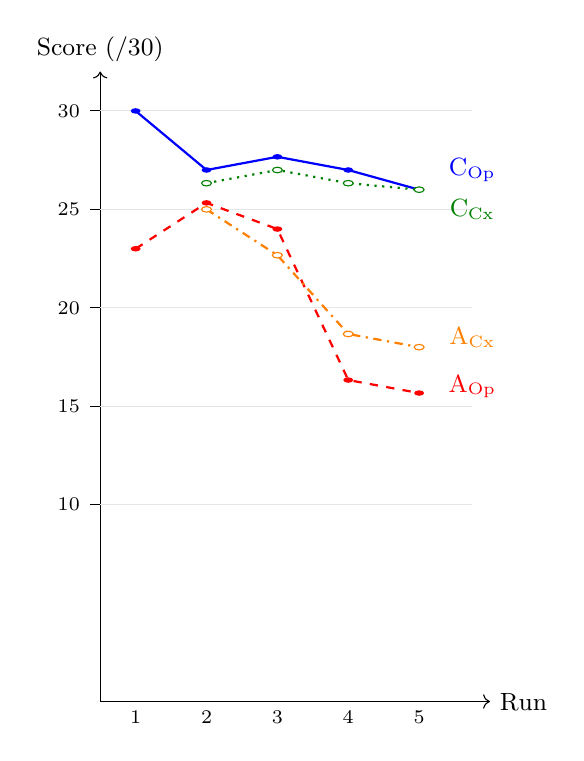
\begin{tikzpicture}[xscale=0.45, yscale=0.25]
\draw[->] (0,0) -- (11,0) node[right, font=\small] {Run};
\draw[->] (0,0) -- (0,32) node[above, font=\small] {Score (/30)};
\foreach \y in {10,15,20,25,30} {
    \draw (0,\y) -- (-0.3,\y) node[left, font=\scriptsize] {\y};
    \draw[gray!20] (0,\y) -- (10.5,\y);
}
% Opus lines (solid)
\draw[blue, thick] (1,30) -- (3,27) -- (5,27.67) -- (7,27) -- (9,26);
\foreach \x/\y in {1/30, 3/27, 5/27.67, 7/27, 9/26} {
    \fill[blue] (\x,\y) circle (4pt);
}
\node[blue, font=\small] at (10.5,27) {C\textsubscript{Op}};
\draw[red, thick, dashed] (1,23) -- (3,25.33) -- (5,24) -- (7,16.33) -- (9,15.67);
\foreach \x/\y in {1/23, 3/25.33, 5/24, 7/16.33, 9/15.67} {
    \fill[red] (\x,\y) circle (4pt);
}
\node[red, font=\small] at (10.5,16) {A\textsubscript{Op}};
% Codex lines (runs 2--5 only)
\draw[green!50!black, thick, dotted] (3,26.33) -- (5,27.0) -- (7,26.33) -- (9,26.0);
\foreach \x/\y in {3/26.33, 5/27.0, 7/26.33, 9/26.0} {
    \draw[green!50!black, fill=white] (\x,\y) circle (4pt);
}
\node[green!50!black, font=\small] at (10.5,25) {C\textsubscript{Cx}};
\draw[orange, thick, dash dot] (3,25.0) -- (5,22.67) -- (7,18.67) -- (9,18.0);
\foreach \x/\y in {3/25.0, 5/22.67, 7/18.67, 9/18.0} {
    \draw[orange, fill=white] (\x,\y) circle (4pt);
}
\node[orange, font=\small] at (10.5,18.5) {A\textsubscript{Cx}};
\foreach \x/\l in {1/1, 3/2, 5/3, 7/4, 9/5} {
    \node[below, font=\scriptsize] at (\x,0) {\l};
}
\end{tikzpicture}
\caption{ICLR 2025: per-run total scores under Opus (solid) and Codex (dotted) judges. Condition~C is stable under both judge families; Condition~A shows bimodal variance.}
\label{fig:variance}
\end{figure}

\begin{table}[h]
\caption{ICLR 2025: per-run mean scores by dimension (runs 2--5, 3 judges each).}
\label{tab:iclr_detail}
\begin{center}
\begin{tabular}{lcccccccc}
\toprule
& \multicolumn{2}{c}{\textbf{Run 2}} & \multicolumn{2}{c}{\textbf{Run 3}} & \multicolumn{2}{c}{\textbf{Run 4}} & \multicolumn{2}{c}{\textbf{Run 5}} \\
\cmidrule(lr){2-3} \cmidrule(lr){4-5} \cmidrule(lr){6-7} \cmidrule(lr){8-9}
\textbf{Dimension} & A & C & A & C & A & C & A & C \\
\midrule
Cross-abstract inf.  & 5.00 & 5.00 & 4.67 & 5.00 & 3.33 & 5.00 & 3.00 & 5.00 \\
Epistemic strat. & 4.00 & 4.67 & 3.67 & 4.67 & 2.33 & 4.00 & 2.00 & 4.00 \\
Falsifiability   & 3.67 & 4.00 & 3.33 & 4.00 & 2.00 & 4.00 & 2.00 & 4.00 \\
Corpus coverage  & 4.67 & 4.33 & 4.67 & 5.00 & 4.33 & 4.00 & 4.00 & 4.00 \\
Assumption surf. & 4.00 & 5.00 & 4.00 & 5.00 & 2.33 & 5.00 & 2.67 & 5.00 \\
Decision-ready   & 4.00 & 4.00 & 3.67 & 4.00 & 2.00 & 5.00 & 2.00 & 4.00 \\
\midrule
\textbf{Total}   & 25.33 & 27.00 & 24.00 & 27.67 & 16.33 & 27.00 & 15.67 & 26.00 \\
\bottomrule
\end{tabular}
\end{center}
\end{table}

\begin{table}[h]
\caption{AUSA 2025: per-dimension AI judge scores (3 runs, 3 judges).}
\label{tab:ausa_detail}
\begin{center}
\begin{tabular}{lcc}
\toprule
\textbf{Dimension} & \textbf{Cond.\ A} & \textbf{Cond.\ C} \\
\midrule
Cross-abstract inference & 4.00 & 5.00 \\
Epistemic stratification & 3.44 & 5.00 \\
Falsifiability yield & 2.78 & 4.44 \\
Corpus coverage & 5.00 & 4.00 \\
Assumption surfacing & 3.00 & 5.00 \\
Decision-readiness & 3.00 & 4.11 \\
\midrule
\textbf{Total} & 21.22 & 27.56 \\
\bottomrule
\end{tabular}
\end{center}
\end{table}

\section{Blinded Textual Analysis}
\label{app:textual}

Blinded analysis of output characteristics confirms that the conditions produce systematically different text, distinguishable from automated metrics alone (10/10 correct classification on AAHS, 9/10 on ICLR using bigram Jaccard and lexical diversity).

\paragraph{Evidence diversification.} Baseline outputs converge more on citations than pipeline outputs (A--A citation Jaccard = 0.483 vs.\ C--C = 0.432 on AAHS). The pipeline diversifies both evidence selection and phrasing. Within-seed A--C similarity (0.090) is essentially identical to cross-seed A--C similarity (0.093), indicating the pipeline samples from an independent distribution.

\paragraph{Epistemic hygiene.} Pipeline outputs show fewer threshold/data-parroting claims ($-$24\%), more uncertainty markers (+63\%), and more counterfactual reasoning (+53\%).

\paragraph{Faithfulness.} Neither condition fabricates findings. The pipeline shows higher cite-per-claim ratios (3.42 vs.\ 2.29 on AAHS).

\begin{table}[h]
\caption{Group-average similarity metrics across AAHS 5-seed replication (10 responses, 45 pairs).}
\label{tab:similarity}
\begin{center}
\begin{tabular}{lcccc}
\toprule
\textbf{Metric} & \textbf{A--A} & \textbf{C--C} & \textbf{A--C (within)} & \textbf{A--C (cross)} \\
\midrule
Cosine similarity & 0.952 & 0.950 & 0.900 & 0.905 \\
Unigram Jaccard & 0.452 & 0.387 & 0.356 & 0.365 \\
Bigram Jaccard & 0.150 & 0.100 & 0.090 & 0.093 \\
Citation Jaccard & 0.483 & 0.432 & 0.330 & 0.338 \\
\bottomrule
\end{tabular}
\end{center}
\end{table}

\section{Example Synthesis Openings}
\label{app:examples}

The following excerpts illustrate the difference in register between baseline and pipeline outputs (AAHS 2026, Run~1).

\paragraph{Condition A (baseline).}
\begin{quote}
``These 218 abstracts---82 podium presentations and 136 ePosters---paint a detailed portrait of where hand surgery stands in early 2026. The collection is dominated by large-database retrospective studies (TriNetX, PearlDiver, NSQIP, Epic Cosmos), biomechanical cadaveric work, and systematic reviews, with a smaller but notable set of prospective trials and novel technology evaluations. The field is clearly in a phase of consolidation and optimization: refining existing procedures, mining administrative data for risk factors and disparities, and beginning to integrate AI and digital tools into both diagnosis and rehabilitation.''
\end{quote}

\paragraph{Condition C (pipeline).}
\begin{quote}
``This corpus of 218 abstracts from the AAHS 2026 Annual Meeting is not just a collection of studies. It is a portrait of hand surgery's research ecosystem in a particular moment---one defined by the convergence of massive administrative databases, retrospective designs, and a publication incentive structure that rewards volume over depth. What emerges, when you read all 218 as a single document rather than 218 individual papers, is a field that has become extraordinarily efficient at generating publishable results while leaving its most important questions unaddressed.''
\end{quote}

Condition~A adopts a descriptive, survey-oriented stance; Condition~C immediately interrogates the research ecosystem itself. AI judges consistently scored the latter higher on epistemic stratification and assumption surfacing; the domain expert found both ``similar.''

\section{Detailed Human Expert Feedback}
\label{app:human_detail}

\subsection{Defense Policy (AUSA 2025)}

The reviewer scored both outputs on 5 practitioner-oriented dimensions (1--5 scale) and provided extensive qualitative feedback. The pipeline's interpretive additions were perceived as obvious to a domain insider:

\begin{quote}
``Of course AUSA does advocacy. Of course nobody says China is the adversary. Of course they don't talk about DOGE and piss off the admin. Of course they don't interview soldier spouses.''
\end{quote}

The reviewer's overall assessment: if the interpretation is bad, ``I only want the facts, and the naive one sticks to the facts.'' The pipeline's assumption surfacing---its strongest dimension by AI judge scores---was perceived as stating field-obvious truths. The gaps flagged by the pipeline ``aren't the ones that an expert would want flagged from the material.''

\subsection{Hand Surgery (AAHS 2026)}

The hand surgeon read both outputs and reported: ``honestly the 2 were similar. It will take a deeper dive to discern major differences.''

On the content itself:
\begin{quote}
``Major discussion topics: Declining reimbursement, peri-operative medications, WALANT economics, IM fixation and Socioeconomic impacts. Nothing new or informative for me. I tend to be ahead of the curve when it comes to emerging technologies. It serves as a reinforcement of what I presumed to be, so in that sense it is informative.''
\end{quote}

The reviewer confirmed that the corpus captured the right themes but found neither output provided information beyond what he already knew.

\subsection{Machine Learning (ICLR 2025)}

The active ML researcher read both outputs and reported: ``One isn't obviously `better' than the other.'' Differences were ``mostly about taste'' once factual accuracy was assumed.

\paragraph{Valued.} ``I liked the way that the prose for shape of the field was structured, that it provided the big themes before diving in.'' Thematic consistency built trust: ``None of its contents were thematically surprising to me, which built trust.'' Cross-cutting themes and concise bullet-list formatting were positively received.

\paragraph{Critiqued as obvious.} Trajectory and implications: ``mostly obvious conclusions.'' Methodological observations: ``pretty obvious. It'd be more interesting to contrast with the past and flag opportunities.'' Overall: ``If I were an `active' researcher I don't know if I'd have found them helpful beyond it being a cute summarization.''

\paragraph{Wanted but absent.} The reviewer articulated capabilities absent from both conditions:
\begin{itemize}
    \item Hyperlinks to specific papers or OpenReview IDs.
    \item Outlier highlighting: ``I'd have wanted it to highlight the `weird' and therefore possibly more interesting papers.''
    \item Personalized relevance filtering: ``The even more powerful thing would be to let each researcher rapidly shape the relevance landscape of the thematic analysis based on their research interests.''
    \item Quality-based filtering by institution, methods rigor, etc.
    \item Temporal comparison: ``Rather than underrepresented areas, it'd have been more interesting to contrast the thematic analysis of this year with last year.''
    \item Normative transparency: ``Notable individual contributors should have offered a rationale for why those specific ones were picked.''
    \item Raw analytical artifacts: ``It'd almost be helpful to have excavate or ramify outputs on the corpus as a whole. I.e., assumptions or predictions.''
\end{itemize}

\paragraph{On the task itself.} ``This is a sort of `summarization' task which is inherently underspecified. So different people will have wildly different preferences than what I'm saying here.''

\section{LLM Usage Statement}
\label{app:llm_usage}

Large language models played a significant role in both the research and the writing of this paper. Claude Opus 4.6 served as (1)~the generation model under study, producing all synthesis outputs in both experimental conditions; (2)~a component of the evaluation apparatus, with Claude Opus 4.6 and GPT-5 (Codex) instances serving as AI judges; and (3)~a drafting and revision assistant for the manuscript text itself. All experimental prompts, evaluation rubrics, and raw model outputs are available for inspection. The research questions, experimental design, domain expert recruitment, and interpretive framing were conducted by the human authors.

\end{document}
